\documentclass[
    12pt,
    a4paper,
    oneside,
    chapter=TITLE,
    section=TITLE,
    subsection=TITLE,
    subsubsection=TITLE,
    english,
    french,
    spanish,
    brazil,
    ]{abntex2}

\usepackage{lmodern}
\usepackage[T1]{fontenc}
\usepackage[utf8]{inputenc}
\usepackage{indentfirst}
\usepackage{color}
\usepackage{graphicx}
\usepackage{microtype}
\usepackage[brazilian,hyperpageref]{backref}
\usepackage[alf]{abntex2cite}

\renewcommand{\backrefpagesname}{Citado na(s) página(s):~}
\renewcommand{\backref}{}
\renewcommand*{\backrefalt}[4]{
    \ifcase #1
        Nenhuma citação no texto.
    \or
        Citado na página #2.
    \else
        Citado #1 vezes nas páginas #2.
    \fi}

\titulo{NOME DO PROJETO}
\autor{DDLS}
\local{Campina Grande}
\data{\today}
\instituicao{
  \textbf{Statement of Work}
  \par
  Instituto Federal de Educação, Ciência e Tecnologia da Paraíba
  }
\tipotrabalho{Projeto de Pesquisa}
\preambulo{Especificação de projeto feito com objetivo de apresentar e auxiliar o desenvolvimento do mesmo, apresentado à comunidade do IFPB}

\definecolor{blue}{RGB}{41,5,195}
\makeatletter
\hypersetup{
        %pagebackref=true,
        pdftitle={\@title}, 
        pdfauthor={\@author},
        pdfsubject={\imprimirpreambulo},
        pdfcreator={LaTeX with abnTeX2},
        pdfkeywords={abnt}{latex}{abntex}{abntex2}{projeto de pesquisa}, 
        colorlinks=false,               
        linkcolor=blue,             
        citecolor=blue,             
        filecolor=magenta,          
        urlcolor=blue,
        bookmarksdepth=4
}
\makeatother

\setlength{\parindent}{1.3cm}
\setlength{\parskip}{0.2cm}

\makeindex

\begin{document}

\selectlanguage{brazil}
\frenchspacing 
\imprimircapa
\imprimirfolhaderosto

\pdfbookmark[0]{\contentsname}{toc}
\tableofcontents*
\cleardoublepage

\textual

\chapter{Problema}

\chapter{Interface}

A interface de comunicação do seu sistema deve atender os seguintes requisitos da \autoref{tabela-interface}:

\begin{table}[htb]
\IBGEtab{
  \caption{Especificação de Dados}
  \label{tabela-interface}
}{
  \begin{tabular}{ccc}
  \toprule
   Nome & Tipo & Tamanho em bits \\
  \midrule \midrule
   Valid & Entrada & 1 \\
  \midrule 
   DataIn & Entrada & 32 \\
  \midrule 
   Ready & Saída & 1 \\
  \midrule 
   DataOut & Saída & 32 \\
  \bottomrule
\end{tabular}
}{
  \fonte{Produzido pelos autores.}%
  \nota{Ready será levado para 1 quando o IP estiver pronto para entrada ou saída de dados.}
  \nota{Valid só será ativado quando o ready estiver levantado e servirá para a entrada de dados.}
  \nota{DataIn só será gravado quando o Valid e o Ready estiverem ativos.}
  }
\end{table}

Na \autoref{fig-maquina-estados} você pode analisar a maquina de estados do sistema.
\par
\begin{figure}[htb]
    \caption{\label{fig-maquina-estados}Maquina de Estados da Interface}
    \begin{center}
        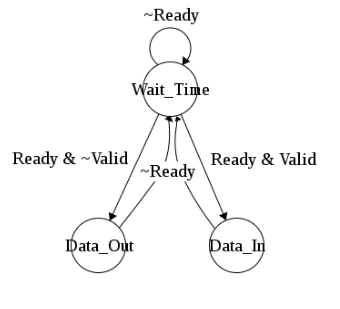
\includegraphics[scale=0.8]{imgs/maquina-estados.png}
    \end{center}
    \legend{Fonte: Produzido pelos autores.}
\end{figure}


\chapter{Entrada}

\chapter{Saída}

\chapter{Caso Base}

\end{document}